%% LyX 2.1.3 created this file.  For more info, see http://www.lyx.org/.
%% Do not edit unless you really know what you are doing.
\documentclass{article}
\usepackage[latin9]{inputenc}
\usepackage{color}
\usepackage{verbatim}
\usepackage{amsmath}
\usepackage{graphicx}

\makeatletter

%%%%%%%%%%%%%%%%%%%%%%%%%%%%%% LyX specific LaTeX commands.
%% Because html converters don't know tabularnewline
\providecommand{\tabularnewline}{\\}

%%%%%%%%%%%%%%%%%%%%%%%%%%%%%% User specified LaTeX commands.
% -----------------------------------------------
% Template for ISMIR Papers
% 2016 version, based on previous ISMIR templates

% Requirements :
% * 6+1 page length maximum
% * 2MB maximum file size
% * Copyright note must appear in the bottom left corner of first page
% (see conference website for additional details)
% -----------------------------------------------

\usepackage{ismir}
\usepackage{cite}

% Title.
% ------
\title{Harmonic Modeling of Singing Voice for Source Separation}

% Note: Please do NOT use \thanks or a \footnote in any of the author markup

% Single address
% To use with only one author or several with the same address
% ---------------
\oneauthor
{Georgi Dzhambazov, Xavier Serra}
{Music Technology Group, Universitat Pompeu Fabra, Barcelona, Spain}

% Two addresses
% --------------
%\twoauthors
%  {First author} {School \\ Department}
%  {Second author} {Company \\ Address}

%% To make customize author list in Creative Common license, uncomment and customize the next line
%  \def\authorname{First Author, Second Author} 


% Three addresses
% --------------
%\threeauthors
% {First Author} {Affiliation1 \\ {\tt author1@ismir.edu}}
% {Second Author} {\bf Retain these fake authors in\\\bf submission to preserve the formatting}
%  {Third Author} {Affiliation3 \\ {\tt author3@ismir.edu}}

%% To make customize author list in Creative Common license, uncomment and customize the next line
%  \def\authorname{First Author, Second Author, Third Author} 

% Four or more addresses
% OR alternative format for large number of co-authors
% ------------
%\multauthor
%{  \hspace{0.6cm}Georgi Dzhambazov\hspace{0.1cm} \\
 % Music Technology Group, Universitat Pompeu Fabra, Barcelona, Spain\\
%$^2$ International Laboratories, City, Country\\
%$^3$  Company, Address\\
%{\tt\small georgi.dzhambazov@upf.edu}}
\def\authorname{Georgi Dzhambazov, Xavier Serra}


\sloppy % please retain sloppy command for improved formatting

\makeatother

\begin{document}
\sloppy

\maketitle 


\section{Introduction}

In this work we suggest how to separate singing voice from an audio
mixture relying on an an approach for harmonic modeling. The idea
of the harmonic model is to represent the spectral content of a predominant
source with harmonic nature as a sum of the fundamental frequency
and its partials. Harmonics are function of input detected pitch contours.
Therefore, a pitfall for detecting singing voice might be pitch segments
coming from soloing instruments with harmonic nature. In \cite{lehner2014reduction}
are suggested a set of timbral features that help discriminate between
regions of singing voice and musical instruments. We filter out instrumental
regions by classifying the harmonic content, based on these features. 

Although vocal modeling could be a conceptual part in some source
separation (SS) approaches \cite{durrieu2011musically}, in most of
them, vocal detection (VD)  is not done as an explicit step. Only
recently it has been shown that VD can enhance the separated signal
as a post-processing step to SS \cite{lehner2015monaural}. 


\section{Approach}

\begin{figure}
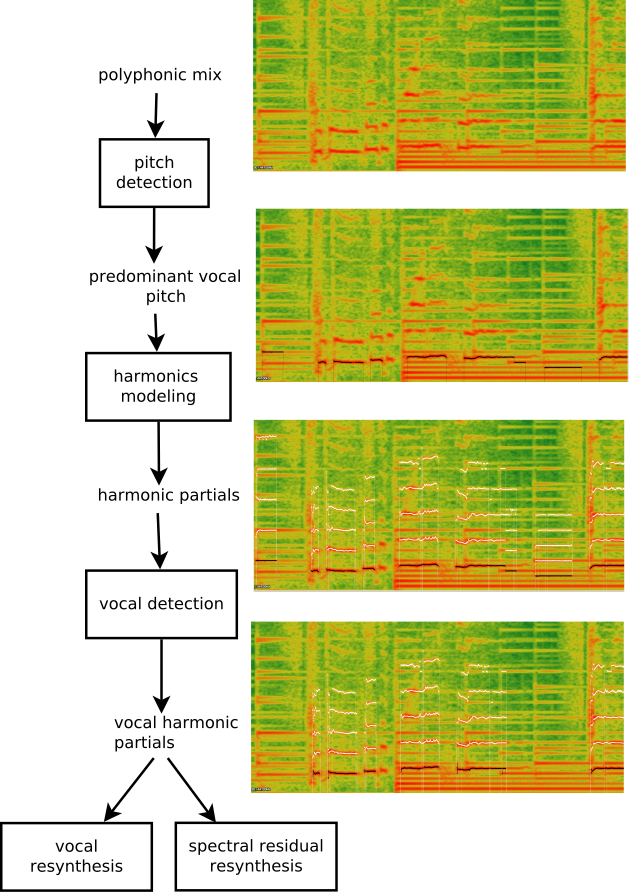
\includegraphics[width=1\columnwidth]{Overview_with_screenShots}

\protect\caption{Overview of approach.}
\end{figure}



\subsection{Pitch detection}

The harmonic modeling requires as input the pitch series of the main
source. We rely on the \emph{Melodia} algorithm\cite{salamon2012melody}
to extract the pitch for time intervals with predominant melodic source
(pitch contours). The methodology computes for each contour how harmonically
salient it is, based on the saliences of each pitch value. Then contours
from the main source are selected as having salience over a threshold
relative to the average mean salience of all contours. We used the
open-source implementation from the feature extraction framework \emph{essentia}\footnote{http://essentia.upf.edu},
in which we have set the voicing threshold to $1.4$, and guessUnvoiced=True
which increased the recall of the vocal regions . A side effect of
that is though, that some instrumental time intervals increase the
false positives rate. 


\subsection{Harmonic modeling}

The harmonic model \cite{Serra89asystem} filters the spectral peaks
corresponding to the first 30 harmonic partials of the singing voice.

\[
Yh[k]=\sum_{r=1}^{R}A_{r}W[k-r\hat{f}_{0}]
\]



\subsection{Vocal detection}

To filter out the regions from background instruments, we have trained
a vocal classifier following the approach of \cite{lehner2014reduction}.
Like them we trained a random forest classifier (100 trees in \emph{scikit-learn})
but used only timbral features: 30 MFCCs and 'vocal variance' (the
variance of the first 5 MFCCs). The motivation is that timbral-based
vocal classification complements the vocal detection approach of \emph{Melodia},
relying only on pitch-contour salience. A frame is classified as voiced
or non-voiced based on majority voting of the trees. %
\begin{comment}
in doit() : if Parameters.WITH\_VOCAL\_DETECTION
\end{comment}
{} Detected non-vocal frames were muted from the estimated voice. 


\subsubsection{Training}

\cite{lehner2015monaural} indicates that VD accuracy of the separated
signal is higher when trained also on separated signal rather than
on the original mix. We trained thus on harmonic partials extracted
from the original mix using all avaialble audio of the \emph{iKala}
dataset of around $125$ minutes\footnote{http://mac.citi.sinica.edu.tw/ikala/description.html}.
The  reference MIDI annotation is used as input to the harmonic model.
\begin{comment}
IMPL.. DETAIL -for each vocal segment or non-vocal segment from annotation
features are extracted as if it were separate audio. This assures
that features with wide timespan (e.g. vocal variance) are extracted
without interference from adjacent regions.
\end{comment}
\begin{comment}
train\_main.get\_class\_frames
\end{comment}



\subsection{Resynthesis}

The vocal source is resynthesized by means of a constant overlap add
resynthesis  with the \emph{sms-tools} package\footnote{http://mtg.upf.edu/technologies/sms}.
Finally the background is derived by multuplying the original mix
by a simple soft mask.

\begin{table}
\begin{tabular}{|c|c|c|}
\hline 
 & before VD & after VD\tabularnewline
\hline 
recall & 0.83 & 0.76\tabularnewline
\hline 
false alarms & 0.35 & 0.22\tabularnewline
\hline 
\end{tabular}

\protect\caption{{\small{}Vocal detection parameters}{\small \par}}
\end{table}





\section{Results}

The proposed approach has been implemented in python\footnote{https://github.com/georgid/vocal-detection}.
Result on the test part of the iKala dataset are summarized in Table
1\footnote{complete results are available on http://www.music-ir.org/mirex/wiki/2016:Singing\_Voice\_Separation\_Results}.

\begin{table}
\begin{centering}
\begin{tabular}{|c|c|c|c|c|}
\hline 
 & \multicolumn{2}{c|}{voice} & \multicolumn{2}{c|}{accompaniment}\tabularnewline
\hline 
 & mean & st dev & mean & st dev\tabularnewline
\hline 
\hline 
NSDR & -2.281 & 3.534 & 0.395 & 1.470\tabularnewline
\hline 
SIR & 6.562 & 9.778 & 1.984 & 9.805\tabularnewline
\hline 
SAR & 2.394 & 4.562 & 2.708 & 2.661\tabularnewline
\hline 
\end{tabular}
\par\end{centering}

\protect\caption{Results measured by source separation metrics: Normalized Signal-to-Distortion
Ratio (NSRD), Signal-to-Interference Ratio (SIR), Signal-to-Artifacts
Ratio (SAR)}
\end{table}



\subparagraph*{Acknowledgements}

\textcolor{black}{We are thankful to Bernhard Lehner for providing
help with running the timbral feature extraction.}\textcolor{red}{{}
}This work is partly supported by the European Research Council under
the European Union\textquoteright s Seventh Framework Program, as
part of the CompMusic project (ERC grant agreement 267583) and partly
by the AGAUR research grant.s

\bibliographystyle{plain}
\bibliography{JabRefSingingVoiceSeparation}


% For non bibtex users:%\begin{thebibliography}{citations}%\bibitem {Author:00}%E. Author.%``The Title of the Conference Paper,''%{\it Proceedings of the International Symposium%on Music Information Retrieval}, pp.~000--111, 2000.%\bibitem{Someone:10}%A. Someone, B. Someone, and C. Someone.%``The Title of the Journal Paper,''%{\it Journal of New Music Research},%Vol.~A, No.~B, pp.~111--222, 2010.%\bibitem{Someone:04} X. Someone and Y. Someone. {\it Title of the Book},%    Editorial Acme, Porto, 2012.%\end{thebibliography}
\end{document}
